% GNUPLOT: LaTeX picture with Postscript
\begingroup
  % Encoding inside the plot.  In the header of your document, this encoding
  % should to defined, e.g., by using
  % \usepackage[latin1,<other encodings>]{inputenc}
  \inputencoding{latin1}%
  \makeatletter
  \providecommand\color[2][]{%
    \GenericError{(gnuplot) \space\space\space\@spaces}{%
      Package color not loaded in conjunction with
      terminal option `colourtext'%
    }{See the gnuplot documentation for explanation.%
    }{Either use 'blacktext' in gnuplot or load the package
      color.sty in LaTeX.}%
    \renewcommand\color[2][]{}%
  }%
  \providecommand\includegraphics[2][]{%
    \GenericError{(gnuplot) \space\space\space\@spaces}{%
      Package graphicx or graphics not loaded%
    }{See the gnuplot documentation for explanation.%
    }{The gnuplot epslatex terminal needs graphicx.sty or graphics.sty.}%
    \renewcommand\includegraphics[2][]{}%
  }%
  \providecommand\rotatebox[2]{#2}%
  \@ifundefined{ifGPcolor}{%
    \newif\ifGPcolor
    \GPcolortrue
  }{}%
  \@ifundefined{ifGPblacktext}{%
    \newif\ifGPblacktext
    \GPblacktextfalse
  }{}%
  % define a \g@addto@macro without @ in the name:
  \let\gplgaddtomacro\g@addto@macro
  % define empty templates for all commands taking text:
  \gdef\gplbacktext{}%
  \gdef\gplfronttext{}%
  \makeatother
  \ifGPblacktext
    % no textcolor at all
    \def\colorrgb#1{}%
    \def\colorgray#1{}%
  \else
    % gray or color?
    \ifGPcolor
      \def\colorrgb#1{\color[rgb]{#1}}%
      \def\colorgray#1{\color[gray]{#1}}%
      \expandafter\def\csname LTw\endcsname{\color{white}}%
      \expandafter\def\csname LTb\endcsname{\color{black}}%
      \expandafter\def\csname LTa\endcsname{\color{black}}%
      \expandafter\def\csname LT0\endcsname{\color[rgb]{1,0,0}}%
      \expandafter\def\csname LT1\endcsname{\color[rgb]{0,1,0}}%
      \expandafter\def\csname LT2\endcsname{\color[rgb]{0,0,1}}%
      \expandafter\def\csname LT3\endcsname{\color[rgb]{1,0,1}}%
      \expandafter\def\csname LT4\endcsname{\color[rgb]{0,1,1}}%
      \expandafter\def\csname LT5\endcsname{\color[rgb]{1,1,0}}%
      \expandafter\def\csname LT6\endcsname{\color[rgb]{0,0,0}}%
      \expandafter\def\csname LT7\endcsname{\color[rgb]{1,0.3,0}}%
      \expandafter\def\csname LT8\endcsname{\color[rgb]{0.5,0.5,0.5}}%
    \else
      % gray
      \def\colorrgb#1{\color{black}}%
      \def\colorgray#1{\color[gray]{#1}}%
      \expandafter\def\csname LTw\endcsname{\color{white}}%
      \expandafter\def\csname LTb\endcsname{\color{black}}%
      \expandafter\def\csname LTa\endcsname{\color{black}}%
      \expandafter\def\csname LT0\endcsname{\color{black}}%
      \expandafter\def\csname LT1\endcsname{\color{black}}%
      \expandafter\def\csname LT2\endcsname{\color{black}}%
      \expandafter\def\csname LT3\endcsname{\color{black}}%
      \expandafter\def\csname LT4\endcsname{\color{black}}%
      \expandafter\def\csname LT5\endcsname{\color{black}}%
      \expandafter\def\csname LT6\endcsname{\color{black}}%
      \expandafter\def\csname LT7\endcsname{\color{black}}%
      \expandafter\def\csname LT8\endcsname{\color{black}}%
    \fi
  \fi
    \setlength{\unitlength}{0.0500bp}%
    \ifx\gptboxheight\undefined%
      \newlength{\gptboxheight}%
      \newlength{\gptboxwidth}%
      \newsavebox{\gptboxtext}%
    \fi%
    \setlength{\fboxrule}{0.5pt}%
    \setlength{\fboxsep}{1pt}%
\begin{picture}(8502.00,5102.00)%
    \gplgaddtomacro\gplbacktext{%
      \csname LTb\endcsname%%
      \put(946,704){\makebox(0,0)[r]{\strut{}$0.09$}}%
      \put(946,1226){\makebox(0,0)[r]{\strut{}$0.1$}}%
      \put(946,1748){\makebox(0,0)[r]{\strut{}$0.11$}}%
      \put(946,2270){\makebox(0,0)[r]{\strut{}$0.12$}}%
      \put(946,2792){\makebox(0,0)[r]{\strut{}$0.13$}}%
      \put(946,3315){\makebox(0,0)[r]{\strut{}$0.14$}}%
      \put(946,3837){\makebox(0,0)[r]{\strut{}$0.15$}}%
      \put(946,4359){\makebox(0,0)[r]{\strut{}$0.16$}}%
      \put(946,4881){\makebox(0,0)[r]{\strut{}$0.17$}}%
      \put(1397,484){\makebox(0,0){\strut{}$2.29$}}%
      \put(2994,484){\makebox(0,0){\strut{}$2.295$}}%
      \put(4591,484){\makebox(0,0){\strut{}$2.3$}}%
      \put(6189,484){\makebox(0,0){\strut{}$2.305$}}%
      \put(7786,484){\makebox(0,0){\strut{}$2.31$}}%
    }%
    \gplgaddtomacro\gplfronttext{%
      \csname LTb\endcsname%%
      \put(198,2792){\rotatebox{-270}{\makebox(0,0){\strut{}$\langle |L| \rangle$}}}%
      \put(4591,154){\makebox(0,0){\strut{}$\beta$}}%
      \csname LTb\endcsname%%
      \put(7118,4708){\makebox(0,0)[r]{\strut{}Nur Metropolis Updates: Daten}}%
      \csname LTb\endcsname%%
      \put(7118,4488){\makebox(0,0)[r]{\strut{}Metropolis und Overrelaxation Updates: Daten}}%
      \csname LTb\endcsname%%
      \put(7118,4268){\makebox(0,0)[r]{\strut{}Nur Metropolis Updates: Anpassung $\chi^2=\num{1.26}$}}%
      \csname LTb\endcsname%%
      \put(7118,4048){\makebox(0,0)[r]{\strut{}Metropolis und Overrelaxation Updates: Anpassung $\chi^2=\num{1.85}$}}%
      \csname LTb\endcsname%%
      \put(-777959,69102){\makebox(0,0)[l]{\strut{}reduziertes $\chi^2 = \num{2.53}$}}%
    }%
    \gplbacktext
    \put(0,0){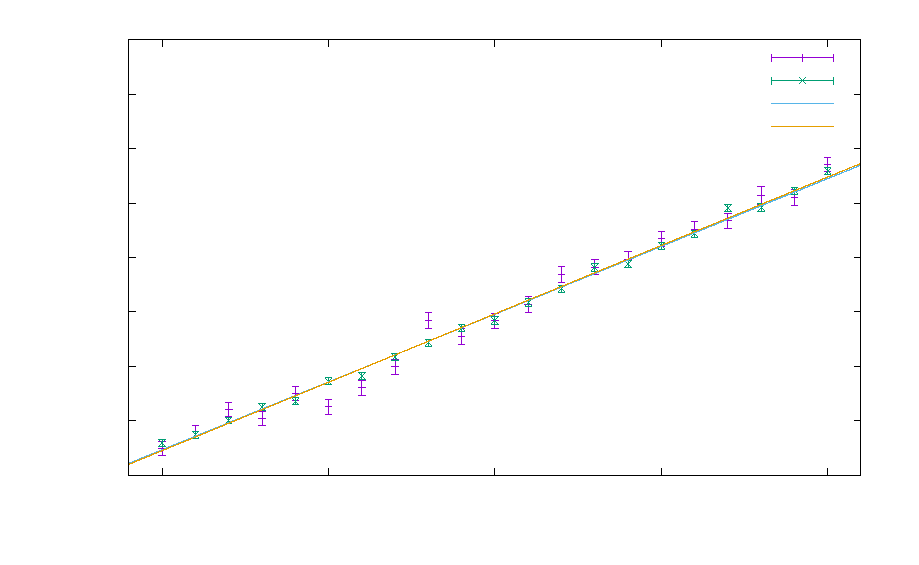
\includegraphics{overr_metropolis_comp}}%
    \gplfronttext
  \end{picture}%
\endgroup
